\documentclass[letterpaper]{article}
%\documentclass[a5paper]{article}

%% Language and font encodings
\usepackage[english]{babel}
\usepackage[utf8x]{inputenc}
\usepackage[T1]{fontenc}

%% Sets page size and margins
\usepackage[letterpaper,top=1in,bottom=1in,left=1in,right=1in,marginparwidth=1.75cm]{geometry}
%\usepackage[a5paper,top=1cm,bottom=1cm,left=1cm,right=1.5cm,marginparwidth=1.75cm]{geometry}

%% Useful packages
\usepackage{amssymb, amsmath, amsthm} 
%\usepackage{graphicx}  %%this is currently enabled in the default document, so it is commented out here. 
\usepackage{calrsfs}
\usepackage{braket}
\usepackage{mathtools}
\usepackage{lipsum}
\usepackage{tikz}
\usetikzlibrary{cd}
\usepackage{verbatim}
%\usepackage{ntheorem}% for theorem-like environments
\usepackage{mdframed}%can make highlighted boxes of text
%Use case: https://tex.stackexchange.com/questions/46828/how-to-highlight-important-parts-with-a-gray-background
\usepackage{wrapfig}
\usepackage{centernot}
\usepackage{subcaption}%\begin{subfigure}{0.5\textwidth}
\usepackage{pgfplots}
\pgfplotsset{compat=1.13}
\usepackage[colorinlistoftodos]{todonotes}
\usepackage[colorlinks=true, allcolors=blue]{hyperref}
\usepackage{xfrac}					%to make slanted fractions \sfrac{numerator}{denominator}
\usepackage{enumitem}            
    %syntax: \begin{enumerate}[label=(\alph*)]
    %possible arguments: f \alph*, \Alph*, \arabic*, \roman* and \Roman*
\usetikzlibrary{arrows,shapes.geometric,fit}

\DeclareMathAlphabet{\pazocal}{OMS}{zplm}{m}{n}
%% Use \pazocal{letter} to typeset a letter in the other kind 
%%  of math calligraphic font. 

%% This puts the QED block at the end of each proof, the way I like it. 
\renewenvironment{proof}{{\bfseries Proof}}{\qed}
\makeatletter
\renewenvironment{proof}[1][\bfseries \proofname]{\par
  \pushQED{\qed}%
  \normalfont \topsep6\p@\@plus6\p@\relax
  \trivlist
  %\itemindent\normalparindent
  \item[\hskip\labelsep
        \scshape
    #1\@addpunct{}]\ignorespaces
}{%
  \popQED\endtrivlist\@endpefalse
}
\makeatother

%% This adds a \rewnewtheorem command, which enables me to override the settings for theorems contained in this document.
\makeatletter
\def\renewtheorem#1{%
  \expandafter\let\csname#1\endcsname\relax
  \expandafter\let\csname c@#1\endcsname\relax
  \gdef\renewtheorem@envname{#1}
  \renewtheorem@secpar
}
\def\renewtheorem@secpar{\@ifnextchar[{\renewtheorem@numberedlike}{\renewtheorem@nonumberedlike}}
\def\renewtheorem@numberedlike[#1]#2{\newtheorem{\renewtheorem@envname}[#1]{#2}}
\def\renewtheorem@nonumberedlike#1{  
\def\renewtheorem@caption{#1}
\edef\renewtheorem@nowithin{\noexpand\newtheorem{\renewtheorem@envname}{\renewtheorem@caption}}
\renewtheorem@thirdpar
}
\def\renewtheorem@thirdpar{\@ifnextchar[{\renewtheorem@within}{\renewtheorem@nowithin}}
\def\renewtheorem@within[#1]{\renewtheorem@nowithin[#1]}
\makeatother

%% This makes theorems and definitions with names show up in bold, the way I like it. 
\makeatletter
\def\th@plain{%
  \thm@notefont{}% same as heading font
  \itshape % body font
}
\def\th@definition{%
  \thm@notefont{}% same as heading font
  \normalfont % body font
}
\makeatother

%===============================================
%==============Shortcut Commands================
%===============================================
\newcommand{\ds}{\displaystyle}
\newcommand{\B}{\mathcal{B}}
\newcommand{\C}{\mathbb{C}}
\newcommand{\F}{\mathbb{F}}
\newcommand{\N}{\mathbb{N}}
\newcommand{\R}{\mathbb{R}}
\newcommand{\Q}{\mathbb{Q}}
\newcommand{\T}{\mathcal{T}}
\newcommand{\Z}{\mathbb{Z}}
\renewcommand\qedsymbol{$\blacksquare$}
\newcommand{\qedwhite}{\hfill\ensuremath{\square}}
\newcommand*\conj[1]{\overline{#1}}
\newcommand*\closure[1]{\overline{#1}}
\newcommand*\mean[1]{\overline{#1}}
%\newcommand{\inner}[1]{\left< #1 \right>}
\newcommand{\inner}[2]{\left< #1, #2 \right>}
\newcommand{\powerset}[1]{\pazocal{P}(#1)}
%% Use \pazocal{letter} to typeset a letter in the other kind 
%%  of math calligraphic font. 
\newcommand{\cardinality}[1]{\left| #1 \right|}
\newcommand{\domain}[1]{\mathcal{D}(#1)}
\newcommand{\image}{\text{Im}}
\newcommand{\inv}[1]{#1^{-1}}
\newcommand{\preimage}[2]{#1^{-1}\left(#2\right)}
\newcommand{\script}[1]{\mathcal{#1}}


\newenvironment{highlight}{\begin{mdframed}[backgroundcolor=gray!20]}{\end{mdframed}}

\DeclarePairedDelimiter\ceil{\lceil}{\rceil}
\DeclarePairedDelimiter\floor{\lfloor}{\rfloor}

%===============================================
%===============My Tikz Commands================
%===============================================
\newcommand{\drawsquiggle}[1]{\draw[shift={(#1,0)}] (.005,.05) -- (-.005,.02) -- (.005,-.02) -- (-.005,-.05);}
\newcommand{\drawpoint}[2]{\draw[*-*] (#1,0.01) node[below, shift={(0,-.2)}] {#2};}
\newcommand{\drawopoint}[2]{\draw[o-o] (#1,0.01) node[below, shift={(0,-.2)}] {#2};}
\newcommand{\drawlpoint}[2]{\draw (#1,0.02) -- (#1,-0.02) node[below] {#2};}
\newcommand{\drawlbrack}[2]{\draw (#1+.01,0.02) --(#1,0.02) -- (#1,-0.02) -- (#1+.01,-0.02) node[below, shift={(-.01,0)}] {#2};}
\newcommand{\drawrbrack}[2]{\draw (#1-.01,0.02) --(#1,0.02) -- (#1,-0.02) -- (#1-.01,-0.02) node[below, shift={(+.01,0)}] {#2};}

%***********************************************
%**************Start of Document****************
%***********************************************

%===============================================
%===============Theorem Styles==================
%===============================================

%================Default Style==================
\theoremstyle{plain}% is the default. it sets the text in italic and adds extra space above and below the \newtheorems listed below it in the input. it is recommended for theorems, corollaries, lemmas, propositions, conjectures, criteria, and (possibly; depends on the subject area) algorithms.
\newtheorem{theorem}{Theorem}
\numberwithin{theorem}{section} %This sets the numbering system for theorems to number them down to the {argument} level. I have it set to number down to the {section} level right now.
\newtheorem*{theorem*}{Theorem} %Theorem with no numbering
\newtheorem{corollary}[theorem]{Corollary}
\newtheorem*{corollary*}{Corollary}
\newtheorem{conjecture}[theorem]{Conjecture}
\newtheorem{lemma}[theorem]{Lemma}
\newtheorem*{lemma*}{Lemma}
\newtheorem{proposition}[theorem]{Proposition}
\newtheorem*{proposition*}{Proposition}
\newtheorem{problemstatement}[theorem]{Problem Statement}


%==============Definition Style=================
\theoremstyle{definition}% adds extra space above and below, but sets the text in roman. it is recommended for definitions, conditions, problems, and examples; i've alse seen it used for exercises.
\newtheorem{definition}[theorem]{Definition}
\newtheorem*{definition*}{Definition}
\newtheorem{condition}[theorem]{Condition}
\newtheorem{problem}[theorem]{Problem}
\newtheorem{example}[theorem]{Example}
\newtheorem*{example*}{Example}
\newtheorem*{counterexample*}{Counterexample}
\newtheorem*{romantheorem*}{Theorem} %Theorem with no numbering
\newtheorem{exercise}{Exercise}
\numberwithin{exercise}{section}
\newtheorem{algorithm}[theorem]{Algorithm}

%================Remark Style===================
\theoremstyle{remark}% is set in roman, with no additional space above or below. it is recommended for remarks, notes, notation, claims, summaries, acknowledgments, cases, and conclusions.
\newtheorem{remark}[theorem]{Remark}
\newtheorem*{remark*}{Remark}
\newtheorem{notation}[theorem]{Notation}
\newtheorem*{notation*}{Notation}
%\newtheorem{claim}[theorem]{Claim}  %%use this if you ever want claims to be numbered
\newtheorem*{claim}{Claim}



\pgfplotsset{compat=1.13}

\title{Math 462 - Advanced Linear Algebra \linebreak
	Homework 1}
\author{Trevor Klar}

\begin{document}

\maketitle

\begin{proposition*}\emph{\textbf{(1-2)}} Let there be given functions $f:S \to T$ and $g:T \to U$. Then 
\begin{enumerate}[label=(\roman*)]
\setcounter{enumi}{4}
\item if $g \circ f$ is surjective, then so is $g$. 
\begin{proof}
Since $g \circ f$ is surjective, then for any $y \in U$, there exists an $x \in S$ such that $g \circ f(x) = y$. Now $x$ is in the domain of $f$, so $f(x)$ is in the domain of $g$, and by definition, $g(f(x))=g \circ f(x)=y$. Thus, for any $y \in U$, there exists $f(x) \in T$ such that $g(f(x))=y$, so $g$ is surjective.
\end{proof}
\end{enumerate}	
\end{proposition*}

\noindent \textbf{Exercises:}
\begin{enumerate}
\item Find sets $S$, $T$, and $U$ and functions $f:S \to T$ and $g: T \to U$ such that $g \circ f$ is injective, but $g$ is \emph{not} injective. (\emph{Hint}: The choice of $S=\{0\}$, $T=\{0,1\}$, and $U=\{0\}$ will inevitably lead to the desired result.)
\begin{example*}
Consider the following functions $f:S \to T$ and $g: T \to U$, whose definition is given by the following figure:
\begin{center}
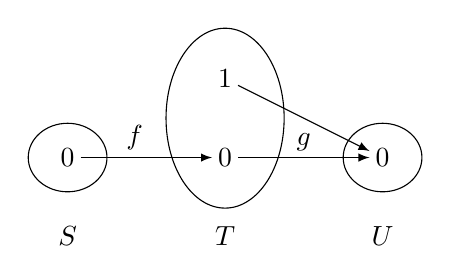
\begin{tikzpicture}
%put some nodes on the left
\foreach \x in {1}{
\node[inner sep=2pt] (s\x) at (0,1-\x) {0};
}
\node[fit=(s1),ellipse,draw,minimum width=1cm] {}; 
%put some nodes on the center
\foreach \x[count=\xi] in {0,1}{
\node[inner sep=2pt] (t\xi) at (2,\x) {\x};
}
\node[fit=(t1) (t2),ellipse,draw,minimum width=1.5cm] {}; 
%put some nodes on the right
\foreach \x[count=\xi] in {1}{
\node[inner sep=2pt] (u\xi) at (4,1-\x) {0};
}
\node[fit=(u1),ellipse,draw,minimum width=1cm] {}; 
%draw the arrows
\draw[-latex] (s1) -- (t1);
\draw[-latex] (t1) -- (u1);
\draw[-latex] (t2) -- (u1);
%label the sets
\node[inner sep=2pt] (setS) at (0,-1) {$S$};
\node[inner sep=2pt] (setT) at (2,-1) {$T$};
\node[inner sep=2pt] (setU) at (4,-1) {$U$};
\node[inner sep=2pt] (funcF) at (.85,0.25) {$f$};
\node[inner sep=2pt] (funcG) at (3,0.2) {$g$};
\end{tikzpicture}
\end{center}
\end{example*}
In this example, $g \circ f$ is injective (vacuously) because for any two $x,y \in S$; $x \neq y \implies g \circ f(x) \neq g \circ f(y)$. This is also more intuitively clear if one recalls that injectivity is also called one-to-one, and since $g \circ f$ contains only the mapping $0 \mapsto 0$, then clearly $g \circ f$ is one-to-one. 

Secondly, $g$ is not injective because $0 \neq 1$, however $g(0)=g(1)=0$. \qed

\item Find sets $S$, $T$, and $U$ and functions $f:S \to T$ and $g: T \to U$ such that $g \circ f$ is surjective, but $f$ is \emph{not} surjective.
\begin{example*}
Actually, the same example for problem (1) will also work for this problem. The composition $g \circ f$ is surjective, because for every $y \in U$ (there is only one), there exists an $x \in S$ such that $g \circ f(x)=y$ ($x=0$). However, $f$ is not surjective because for $y=1$, there does not exist any $x \in S$ such that $f(x)=y$. \qed
\end{example*}

\item Find a non-identity function $f:\R \to \R$ which is its own inverse function. That is, $f \circ f = 1_\R$ or, equivalently, $f(f(x))=x$ for all real $x$. 
\begin{example*}
Let $f(x)=-x$. Then, for all real $x$, $f(x)=-x$, and $f(f(x))=x$. \qed
\end{example*}

\setcounter{enumi}{4}
\item Find a bijective map from the open interval $(\sfrac{-\pi}{2}, \sfrac{+\pi}{2})$ to the set $\R$ of real numbers. This shows, by the way, that both sets have the same cardinality.
\begin{example*}
Let $f:(\sfrac{-\pi}{2}, \sfrac{+\pi}{2}) \to \R$ be defined as $f(x) = \tan(x) = \frac{\sin(x)}{\cos(x)}$. 

We will now show that $f$ is 1-1 and onto. For any two numbers $x_1, x_2 \in (\sfrac{-\pi}{2}, \sfrac{+\pi}{2})$,
$$x_1 \neq x_2 \implies \tan(x_1) \neq \tan(x_2),$$
since $\tan(x)$ is a strictly increasing function. So, $f$ is 1-1. 

Since $\tan(x)$ for an angle $x$ is also defined as the ratio of the opposite leg to the adjacent leg in a right triangle having one angle $x$, we can show that $f$ is surjective. Let $y$ be any arbitrary real number. Now, construct a right trangle with perpendicular sides of length $y$ and $1$. It follows that this triangle has an angle whose tangent is $y$. Thus, $\forall y \in \R, \exists x \in (\sfrac{-\pi}{2}, \sfrac{+\pi}{2})$ such that $\tan(x)=y$, so $f$ is surjective. \qed 
\end{example*}

\item Explicitly construct a bijective function from the set of integers $\Z$ to the set of even integers $2\Z$. 
\begin{example*}
Let $f:\Z \to 2\Z$ be defined as 
$$f(x) = 2x.$$
By definition of an even integer, for every $y \in 2\Z$, there exists an integer $x$ such that $2x=y$. Therefore, $f$ is surjective.

Secondly, if $x \neq y$, then either $x < y$ or $x > y$. Without loss of generality, call $y$ the greater number, so that $x < y$. By the multiplication property of inequality, $2x < 2y$. Therefore, $2x \neq 2y$. We have shown that $x\neq y \implies 2x \neq 2y$, so $f$ is injective. \qed
\end{example*}
\end{enumerate}

\end{document}